\frame{
  \frametitle{H Trees}
  
  \begin{columns}
    \begin{column}{0.5\textwidth}
    \begin{itemize}
    \item Binary tree fractal!

    \medskip
    
    \item Used in chip design in order to distribute wide reaching nets
  \end{itemize}
  \begin{center}
      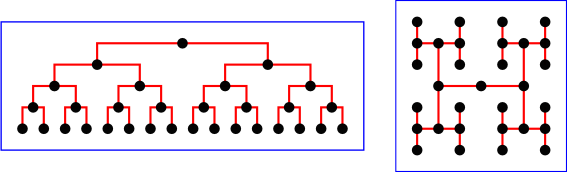
\includegraphics[scale=0.12]{slides/alphabet_trees/HTreeSpace.png}

      {\tiny https://www.tamurajones.net/FractalGenealogy.xhtml}
  \end{center}
    \end{column}
    \begin{column}{0.5\textwidth}
        \begin{center}
         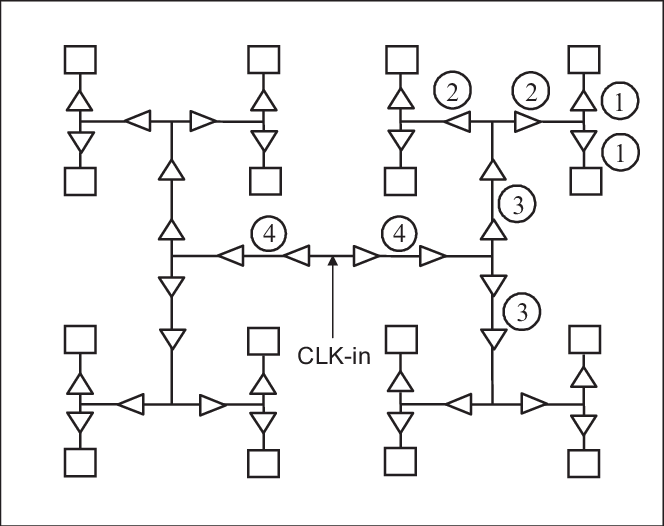
\includegraphics[scale=0.3]{slides/alphabet_trees/An-H-tree-clock-distribution-network-The-index-of-each-level-is-indicated-with-the.png}

         {\tiny Tawfik, Sherif \& Kursun, Volkan. (2008). }
         \end{center}
    \end{column}
    \end{columns}
}
